\documentclass[conference]{IEEEtran}
\IEEEoverridecommandlockouts
% The preceding line is only needed to identify funding in the first footnote. If that is unneeded, please comment it out.
\usepackage{cite}
\usepackage{amsmath,amssymb,amsfonts}
\usepackage{algorithmic}
\usepackage{graphicx}
\usepackage{textcomp}
\usepackage{xcolor}
\usepackage{gensymb}
\def\BibTeX{{\rm B\kern-.05em{\sc i\kern-.025em b}\kern-.08em
    T\kern-.1667em\lower.7ex\hbox{E}\kern-.125emX}}
\begin{document}

\title{RBE 501 Week 2 Assignment}

\author{\IEEEauthorblockN{1\textsuperscript{st} Arjan Gupta}
\IEEEauthorblockA{\textit{Robotics Engineering} \\
\textit{Worcester Polytechnic Institute}\\
Worcester, MA, USA \\
agupta11@wpi.edu}
}

\maketitle

\begin{abstract}
This document provides an in-depth solution for Problems 3--2 and 3--5 described 
in the Robot Modeling and Control textbook.
This is the assignment for the second week in RBE 501 (Robot Dynamics),
Spring 2023 at Worcester Polytechnic Institute.
\end{abstract}

\begin{IEEEkeywords}
robotics, forward kinematics, manipulator
\end{IEEEkeywords}

\section{Introduction}
We are asked to solve Problems 3--2 and 3--5 of the main textbook~\cite{Spong2006}.
For Problem 3--2, the objective is to calculate the forward kinematic equations
of the robot shown in Figure 1 below, \textit{without} using the DH-convention.\\
\begin{figure}[h]
    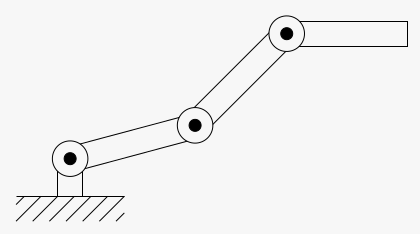
\includegraphics[scale=0.4]{prob3_2.png}
    \centering
    \caption{Three-link planar arm of Problem 3--2}
\end{figure}\\
For Problem 3--5, the objective is to calculate the forward kinematic equations
of the robot shown in Figure 2 below, using the DH-convention.
\begin{figure}[h]
    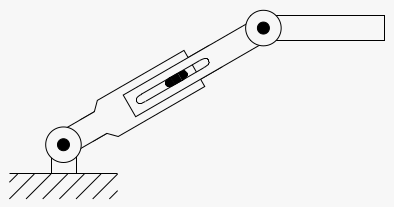
\includegraphics[scale=0.4]{prob3_5.png}
    \centering
    \caption{Three-link planar arm with prismatic joint of Problem 3--5}
\end{figure}

\section{Materials and Methods}

\subsection{Restate objective in technical terms}

We know from the textbook~\cite{Spong2006} that given a rotational matrix $R$, and
a rigid translation $d$, we have the following definition of
a homogeneous transformation,
\[
    H = \begin{bmatrix}
        R & d\\
        0 & 1
    \end{bmatrix}; R \in SO(3), d \in \mathbb{R}^3
\]
Also, the homogeneous transformation $H^m_n$ describes the transformation
of frame $n$ with respect to $m$.
Therefore, given our objectives, and the frames as numbered in Figure 1, 
we need to find $H^0_1$, $H^0_2$, $H^0_3$, and $H^3_2$.

\subsection{Compute all rotation matrices}
As shown in the figure, there are no rotational differences between frames
0, 1, and 2. Therefore, the corresponding rotational matrices are the
$3 \times 3$ identity matrix. So,
\[
    R^0_1 = R^0_2 = I_3 = \begin{bmatrix}
        1 & 0 & 0\\
        0 & 1 & 0\\
        0 & 0 & 1
    \end{bmatrix}
\]
By visually inspecting the figure, we also determine that the rotation for frame 3
can be obtained by a $-180\degree$ rotation around the x-axis, and a
$-90\degree$ rotation around the z-axis. Using our MATLAB Live Script,
we can determine this as,
\[
    R^0_3 = R_{x,-\pi} R_{z,-\frac{\pi}{2}} = \begin{bmatrix}
        0 & 1 & 0\\
        1 & 0 & 0\\
        0 & 0 & -1\\
    \end{bmatrix}
\]
Similarly, the rotation for frame 2 with respect to frame 3 can be obtained
by a $180\degree$ rotation around the y-axis, and a $90\degree$ rotation around
the z-axis. This can be stated as,
\[
    R^3_2 = R_{y,\pi}R_{z,\frac{\pi}{2}} = \begin{bmatrix}
        0 & 1 & 0\\
        1 & 0 & 0\\
        0 & 0 & -1\\
    \end{bmatrix}
\]

\subsection{Compute all the translations}
By visually inspecting the figure, it is easy to see that,
\[
    d^0_1 = \begin{bmatrix}
        0\\
        1\\
        1
    \end{bmatrix}
\]
In order to find $d^0_2$ and $d^0_3$, we need to consider
the geometric distance from frame 0 to the very center of the cube.
In the XY plane, we consider the table top as a square ABCD of side 1,
as shown in Figure 2. Using the geometric properties of a square, we
determine that $AE = EB = 0.5$ because $\triangle AEO \cong \triangle EOB$.

For the Z component of the translations, we need to consider half of the height
of the cube, which is 10 cm, or 0.1 m. Therefore, we can write,
\[
    d^0_2 = \begin{bmatrix}
        -0.5\\
        1.5\\
        1.1
    \end{bmatrix},
    d^0_3 = \begin{bmatrix}
        -0.5\\
        1.5\\
        3
    \end{bmatrix}
\]
Also, since the cube is directly under the camera, we can state,
\[
    d^3_2 = \begin{bmatrix}
        0\\
        0\\
        2
    \end{bmatrix}
\]
\vspace{0.1in}
\section{Results}
Given the fact that we have found all of the rotation matrices and
rigid transformations, we can now form the final results of
our objective. These are as follows,
\[
    H^0_1 = \begin{bmatrix}
        R^0_1 & d^0_1\\
        0 & 1
    \end{bmatrix}
    = \begin{bmatrix}
        1 & 0 & 0 & 0\\
        0 & 1 & 0 & 1\\
        0 & 0 & 1 & 1\\
        0 & 0 & 0 & 1
    \end{bmatrix}
\]
\[
    H^0_2 = \begin{bmatrix}
        R^0_2 & d^0_2\\
        0 & 1
    \end{bmatrix}
    = \begin{bmatrix}
        1 & 0 & 0 & -0.5\\
        0 & 1 & 0 & 1.5\\
        0 & 0 & 1 & 1.1\\
        0 & 0 & 0 & 1
    \end{bmatrix}
\]
\[
    H^0_3 = \begin{bmatrix}
        R^0_3 & d^0_3\\
        0 & 1
    \end{bmatrix}
    = \begin{bmatrix}
        0 & 1 & 0 & -0.5\\
        1 & 0 & 0 & 1.5\\
        0 & 0 & -1 & 3\\
        0 & 0 & 0 & 1
    \end{bmatrix}
\]
\[
    H^3_2 = \begin{bmatrix}
        R^3_2 & d^3_2\\
        0 & 1
    \end{bmatrix}
    = \begin{bmatrix}
        0 & 1 & 0 & 0\\
        1 & 0 & 0 & 0\\
        0 & 0 & -1 & 2\\
        0 & 0 & 0 & 1
    \end{bmatrix}
\]
Furthermore, a MATLAB Live Script has been submitted alongside
this report to show the code used to compute these results.
\section{Discussion}
In the opinion of the author, this problem is very practical
in real-world robotics. If a 3-DOF robotic arm is being operated
(which seems to be the case in Figure 1), then one of the modern 
ways to monitor the arm would be to use computer vision via a camera.
An overhead camera provides a good perspective in such a case, where
the robot perhaps needs to perform tasks on the table-top. Some examples
of table-top tasks could be moving chess pieces, manufacturing assembly,
and other pick-and-place operations. In the case of this problem, the
robot is doing something with a cube.\\
\vspace{0in}\\
Generally, in such a setup, it is imperative to know the relative transformations
between the frames of the robot, table, and the camera in order for a computer
to properly command the controllers of the robot to perform accurate and precise
tasks. For a simple example, if the computer wants to command the robot to go
to a location on the table, first the computer needs to compute that location using
$H^3_1$. Next, the computer needs to use $H^0_1$ to help the robot know about
that location.\\
\vspace{0in}\\
Calibration and frame transformations are very important in order for a robot
to perform any real-world tasks. As for students of robotics, our spatial and
geometric understanding of robotics is tested by this type of problem.
\bibliography{refs.bib}
\bibliographystyle{IEEEtran}

\end{document}